\subsection{Sequential jet-clustering algorithms}
\label{sec:algos}

In this analysis, jets are clustered with sequential jet-clustering algorithms. 
In these algorithms, the four-vectors of input particles are combined pairwise, 
via four-vector addition, until a final jet
is found. Specifically, for each pair of input particles $i$ and $j$,
two quantities are computed, the first is a distance measure between
the two particles, and the second is the so-called ``beam distance''
of each particle:


\begin{eqnarray}
\label{eq:dij}
d_{ij} &=& \mathrm{min}({\pt}_i^{2n},{\pt}_j^{2n}) \Delta R_{ij}^2 / R^2 \\
d_{iB} &=& {\pt}_i^{2n}
\end{eqnarray}

where $\pt$ is the transverse momentum, 
$\Delta R = \sqrt{(\Delta y_{ij})^2 + (\Delta\phi_{ij})^2 }$
is the angular distance between the two particles $i$ and $j$,
and $R$ is an order-unity parameter chosen for the algorithm.
The closest $i,j$ particle pair is combined into a single object, the set of distances is
updated, and the procedure is repeated until the minimum of all the
$d_{ij}$ is greater than the beam distance $d_{iB}$. This is then
classified as a jet and the constituents are removed from further
consideration. The process is repeated until all input four momenta are
clustered. 

The value for $n$ is a parameter of the algorithm in question and
governs the shape of the jets. The different jet algorithms correspond
to different choices of $n$. 
The first such sequential combination algorithm is called the
$k_{\mathrm{T}}$ (KT) algorithm and has $n=1$. These jets are typically irregularly
shaped and are useful for reconstructing lower momentum jets, and is
used to compute the mean $\pt$ per unit area~\cite{ktalg}. 
The second such algorithm
is called the anti-$k_{\mathrm{T}}$ (AK) algorithm and has $n=-1$. This algorithm
behaves like an idealized cone algorithm, and are used extensively
at the LHC experiments and elsewhere~\cite{ktalg}. The third such
algorithm is called the Cambridge-Aachen (CA) algorithm and has $n=0$. This
algorithm uses only angular information, and like the $k_\mathrm{T}$ algorithm
has irregularly-shaped jets. The CA algorithm is very useful for distinguishing
jet substructure~\cite{CAcambridge,CAaachen}.

Jet grooming, $i.e.$ elimination of uncorrelated UE/PU and soft QCD radiation from a target jet, is useful irrespective of the specific 
boosted particle search and can even be applied for soft heavy particles that decay to well-separated jets. 
We consider in this analysis three different forms of grooming: pruning, trimming and filtering. 

%There are choices of what jet algorithm (KT, AK, or CA) can be used by all of these grooming
%algorithms. These algorithms can use different jet algorithms for jet finding and the
%substructure determination. 
These grooming techniques can be applied to jets clustered with different algorithms (KT, AK, or CA).
For the dijet analysis, we have chosen to cluster our jets with the anti-$k_{\mathrm{T}}$
algorithm with $R=0.7$ (AK7), as these are extensively studied at CMS. For the V+jet analysis, in addition to the AK7 jets,  
we study CA jets with $R$=0.8 (CA8), which are used in
recent papers utilizing top-quark tagging~\cite{EXO-11-006}
and $R$=1.2 (CA12), 
which have been proposed for analyses involving boosted
objects~\cite{boostedHiggs}.  
%For the dijet analysis we study the grooming 
%algorithms for the AK7 jets,
%while for the $V+$jets analysis we study them for AK7,
%CA8, and CA12 jets. 
%Comparisons of AK jets with $R=0.5$ (AK5) AND $R=0.8$ (AK8)
%are also investigated, 
%as well as
%with the CA algorithm with $R$=0.8 (CA8) and $R$=1.2 (CA12). 
%The latter
%two are compared because of their usage in other CMS analyses~\cite{EXO-11-006}. 
After the initial jet clustering, the choice of algorithm 
for the substructure determination depends on the algorithm chosen and is described
in detail below. 


\subsection{Filtering algorithm}

The filtering procedure aims to identify relatively hard, symmetric jet splittings that contribute significantly to the jet invariant mass. This procedure is taken from recent Higgs search studies~\cite{boostedHiggs}. The parameters are tuned to maximise sensitivity to a Standard Model Higgs boson decaying to $b\bar{b}$, but this procedure is suitable generally for identifying two-body decay processes. The effect of the procedure is to search for jets where the clustering process combined two relatively low mass objects to make a much more massive object. This indicates the presence of a heavy particle decay. The procedure then attempts to retain only the constituents believed to be related to the decay of this particle.
The identification strategy proposed in~\cite{boostedHiggs} uses the CA algorithm to flexibly adapt to the fact that the two-jet angular separation varies significantly with 
the heavy particle $\pt$ and decay orientation. 
%In this algorithm the angular distance 
%$\Delta R^2_{ij} = (\Delta \eta_{ij} )^2 + (\Delta \phi_{ij} )^2$, 
%where $\eta$ is the pseudorapidity and $\phi$ the azimuthal angle, is calculated between all 
%pairs of objects $i$ and $j$. 
As discussed above, in this algorithm the angular distance $\Delta R^2_{ij}$ is calculated between all pairs of objects $i$ and $j$. 
%The closest pair is combined into a single object, the set of distances is 
%updated, and the procedure is repeated until all objects are separated by a $\Delta R_{ij} > R$, where $R$ 
%is a parameter of the algorithm. 
%This provides a hierarchical structure for the clustering, like the 
%$k_{\mathrm{T}}$ algorithm but in angles rather than in relative transverse momenta.
Each stage in the clustering combines two objects $i$ and $j$ to make another object $k$. 
We use the definition $v = \frac{min({\pt}_i^2,{\pt}_j^2) }{m^2_{k}} \Delta R^2$. The algorithm takes each
jet to be the object $k$ and applies the following sequence:
\begin{enumerate}
\item Undo the last clustering step of $k$ to get $i$ and $j$. These are ordered such that their mass has the property $m_{i} > m_{j}$. If $k$ cannot be unclustered (i.e. it is a single particle) then it is not a suitable candidate for substructure and it is not considered.
\item  If the splitting has $m_{i}/m_{k} < \mu$ (large change in jet mass) and $v > v_{cut}$ (fairly symmetric) then jet $k$ is a suitable substructure candidate and is taken to the next step, otherwise component $i$ is relabeled as $k$ and is taken back to step 1.
Both $\mu$ and $v_{cut}$ are parameters of the algorithm.
\item  Recluster the constituents of the candidate jet with the CA algorithm with an $R$-parameter of $R_{filt} =\mbox{min} (0.3, \Delta R^2_{ij} /2)$ finding $n$ new subjets $s_1, s_2 ...s_n$ ordered in descending $\pt$.
\item  Redefine the jet as the sum of subjet four-momenta $\sum_{i=1}^{min(n,3)} s_i$ or $s_1+s_2$ if $n=2$.
\end{enumerate}


\noindent The algorithm parameters $\mu$ and $v_{cut}$ are taken as 0.67 and 0.09 respectively.
The $\mu$ cut attempts to identify a hard structure in the distribution of energy in the jet, which would imply the decay of a heavy particle. The cut on $v$ further helps by suppressing very asymmetric decays of the type favoured by splittings of quarks and gluons.
Steps 3 and 4 filter out some of the particles in the candidate jet,
the aim being to retain particles relevant to the hard process while
reducing the contribution from effects like underlying event and
pile-up. The 4-vector after step 4 can be treated like a new jet. This
new jet has a $\pt$ and mass less than or equal to those of the
original jet.

As will be demonstrated below, this algorithm is the least aggressive
jet grooming technique. 

\subsection{Trimming algorithm}

Trimming is a technique that ignores particles within a jet that fall below 
a dynamic $\pt$ threshold. It was introduced by Krohn, Thaler and Wang in~\cite{trimming}. 
Trimming reclusters the jets's constituents with the $k_{\mathrm{T}}$ 
algorithm with a radius 
$R_{\rm sub}$ and then accepts only the subjets that have 
%${\pt}_{sub} > f_{cut}$, where $f_{cut}$ is taken proportional 
%either to the jet's $\pt$ or to the event's total $H_T$.
$ {\pt}_{\rm sub} > f_{\rm cut} \lambda_{hard}$ where $f_{cut}$ is a dimensionless parameter, and $\lambda_{\rm hard}$ is some hard scale chosen equal to the seed jet $\pt$. %or the event total transverse momenta $H_{T}$.
The values $R_{\rm sub}$ and $f_{\rm cut}$ are parameters of the algorithm,
taken to be 0.2 and 0.03, respectively. 

As will be demonstrated below, this algorithm is a moderately aggressive
jet grooming technique. 

\subsection{Pruning algorithm}

Pruning was introduced by Ellis, Vermilion and Walsh~\cite{pruning,pruning2}. 
In our implementation, after
the jets are clustered with the original algorithm (either AK7, CA8,
or CA12), the pruning algorithm reclusters the constituents
of the jet with the CA algorithm with the same distance parameter, with extra
veto conditions applied in addition to the standard conditions in Equation~\ref{eq:dij}. 
%The particle is vetoed if either of the following two conditions are met:
The softer of the two particles to be merged is vetoed if both of the following conditions are met:
\begin{eqnarray}
z_{ij} & = & \frac{\mathrm{min}({\pt}_i,{\pt}_j)}{{\pt}_{i+j}} < z_{\mathrm{cut}} \\
\Delta R_{ij} & > & D_{\mathrm{cut}} = \alpha \times \frac{m_J}{{\pt}_J}
\end{eqnarray}
where ${\pt}_i$ and ${\pt}_j$ are the transverse momentum of the constituents,
${\pt}_{i+j}$ is the transverse momentum of the four-vector sum of those constituents,
$m_J$ and ${\pt}_J$ are the mass and transverse momentum of the AK7 jet, 
and $z_{\mathrm{cut}}$ and $\alpha$ are parameters of the algorithm, 
chosen to be 0.1 and 0.5, respectively. 

As will be demonstrated below, this algorithm is the most aggressive
jet grooming technique. 
This algorithm has been previously used for the CMS publication in Ref.~\cite{EXO-11-006}.


\subsection{Groomed jet mass}

Figure~\ref{figs:histAK7PtAvgVsMjetGroomOverReco_ratioPlots}
shows a comparison of the jet mass from the groomed AK7 jets
divided by the jet mass of matched ungroomed AK7 jets, for the
three grooming techniques, for both data and the \PYTHIA Monte Carlo.
As described above, the three different grooming techniques
use different jet algorithms for grooming once the jets are
found with AK7 (CA for filtering and pruning, $k_{\mathrm{T}}$ for trimming).
The data and the MC both exhibit similar behavior. In general,
the filtering algorithm (black) is the least aggressive grooming technique,
with groomed jet masses close to the ungroomed case.
The trimming algorithm (red) is moderately aggressive, and the
pruning algorithm (blue) is the most aggressive. In the case of
the pruning algorithm, the most aggressive technique, a bimodal
distribution begins to manifest,
which is typical of this algorithm since the parameters we have
chosen require two subjets to be created. In the cases where
the pruned jet mass is close to the ungroomed jet mass,
jets usually have large ``core'' components
and small amounts of radiation, whereas when the pruned jet
mass is closer to 0, the jets are more symmetrically split
due to gluons splitting into two jets that fall within
our $D=0.7$ parameter.

\begin{figure}[htbp]
\centering
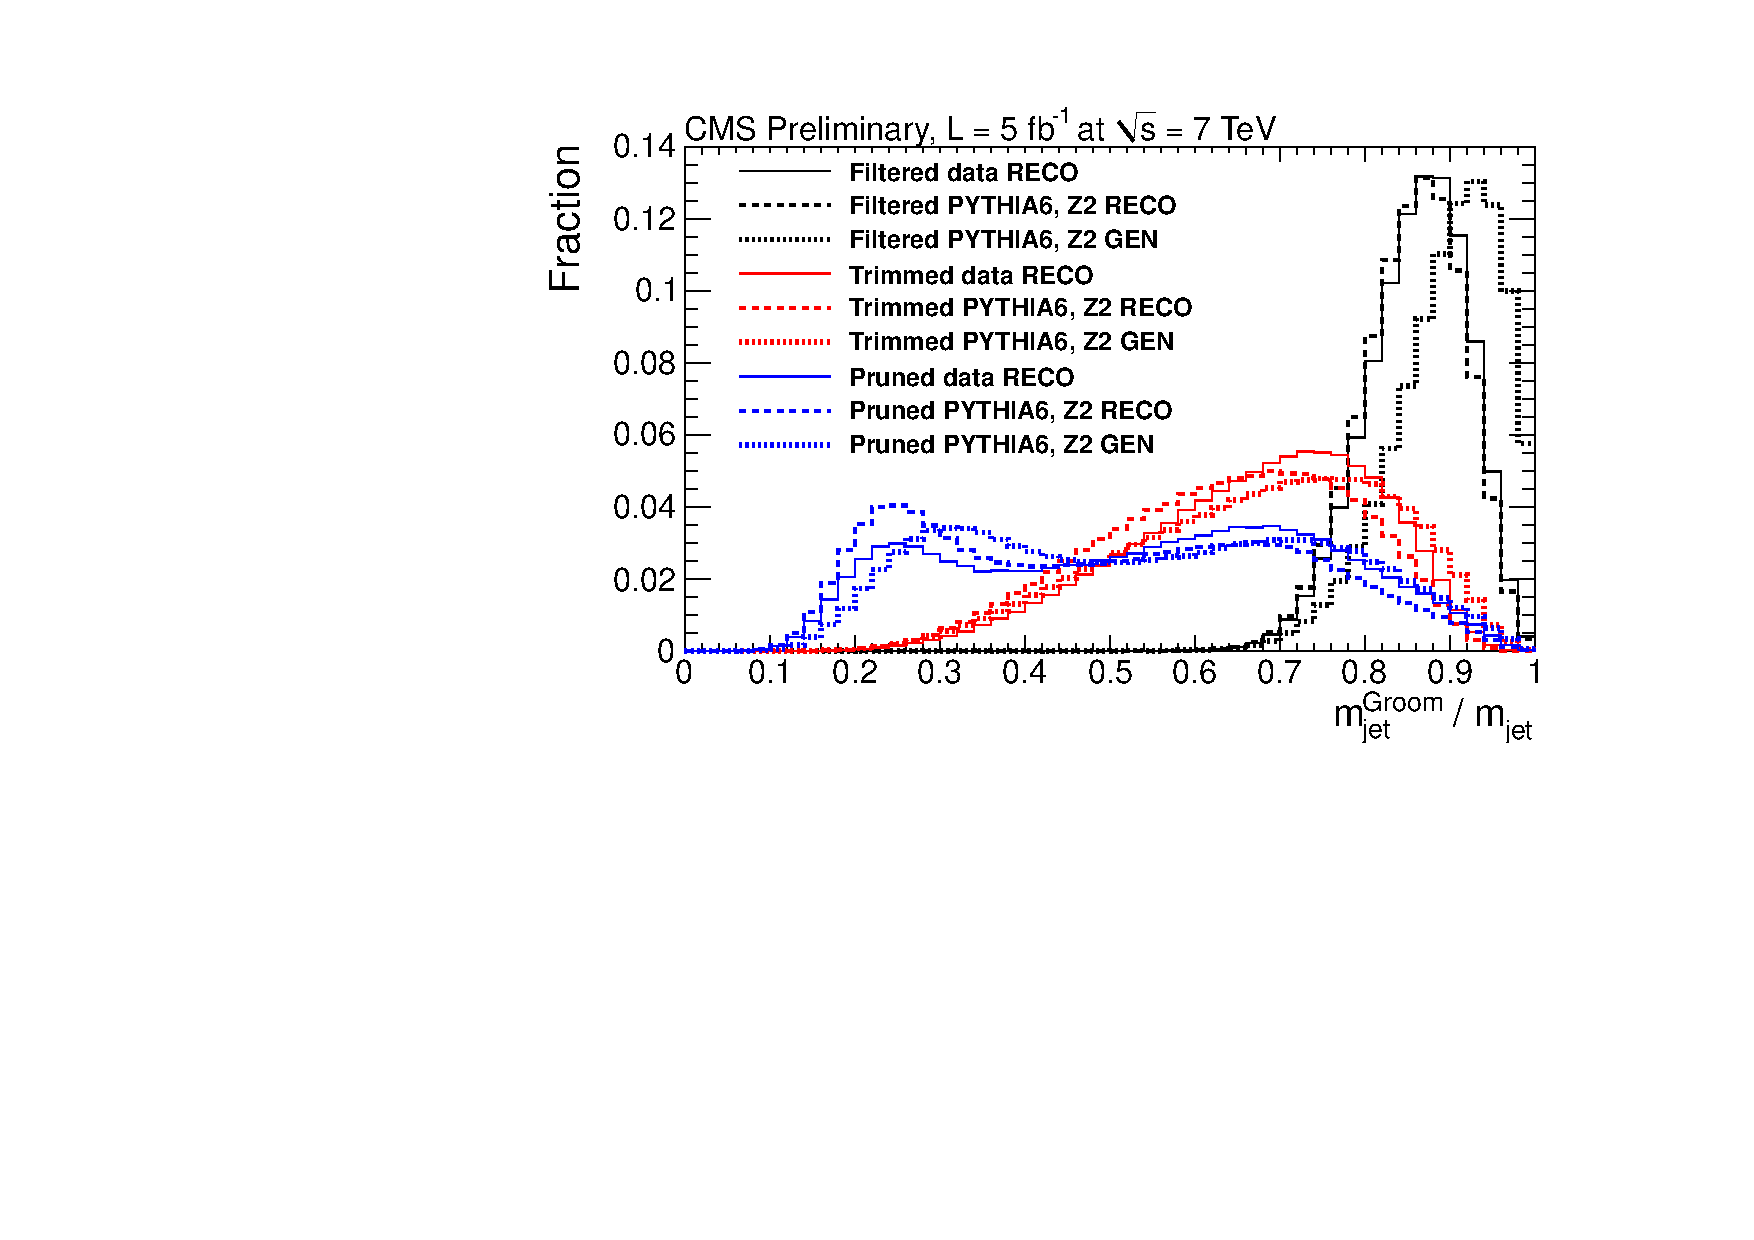
\includegraphics[width=0.95\textwidth]{figs/histAK7PtAvgVsMjetGroomOverReco_ratioPlots}
\caption{Comparison of the jet mass from the groomed jets
divided by the jet mass of matched ungroomed jets for the
three grooming techniques, for both data and the \PYTHIA Monte Carlo.
\label{figs:histAK7PtAvgVsMjetGroomOverReco_ratioPlots}}
\end{figure}





